\documentclass[twoside,a4paper,10pt]{article}
\usepackage[top=2.54cm,bottom=2.54cm,left=2.54cm,right=2.54cm]{geometry}

\usepackage[english]{babel}
\usepackage[utf8]{inputenc}
\usepackage{amsmath}
\usepackage{graphicx}
%\usepackage[colorinlistoftodos]{todonotes}
%\usepackage{url}

\usepackage[hidelinks]{hyperref}
\usepackage{tabularx}
%\usepackage{ref}

%%%

\pagenumbering{arabic}
\usepackage{fancyhdr}

\pagestyle{fancy}
% Shows section number and name
\renewcommand{\sectionmark}[1]{\markright{#1}{}}
% Clear previous styles
\fancyhf{}
\fancyhead{}
\fancyhead[RO]{\thepage}
\fancyhead[LO]{\rightmark}
\fancyhead[RE]{BitTorrent Tracker: deliverable 1}
\fancyhead[LE]{\thepage}
\fancyfoot{}
% Other modifiers
%\fancyfoot[LE,RO]{\thepage}
%\fancyfoot[LO,CE]{Something}
%\fancyfoot[CO,RE]{Author Name}

\title{BitTorrent Tracker: deliverable 1\\
   Group 01}
\author{Irene Díez \and Jesus Sesma}

\begin{document}
\date{}
\maketitle

%\begin{abstract}
%Your abstract.
%\end{abstract}

\section{Architectural design}

Figure~\ref{fig:arch} shows the architectural design of the BitTorrent Tracker.
All swarm member receive UDP multicast requests from the peers; however, just
the master answers.
The communication between the peers is done via UDP, and the
tracker's instances contemplate UDP/JMS communication among them.

\begin{figure}[h]
  \centering
  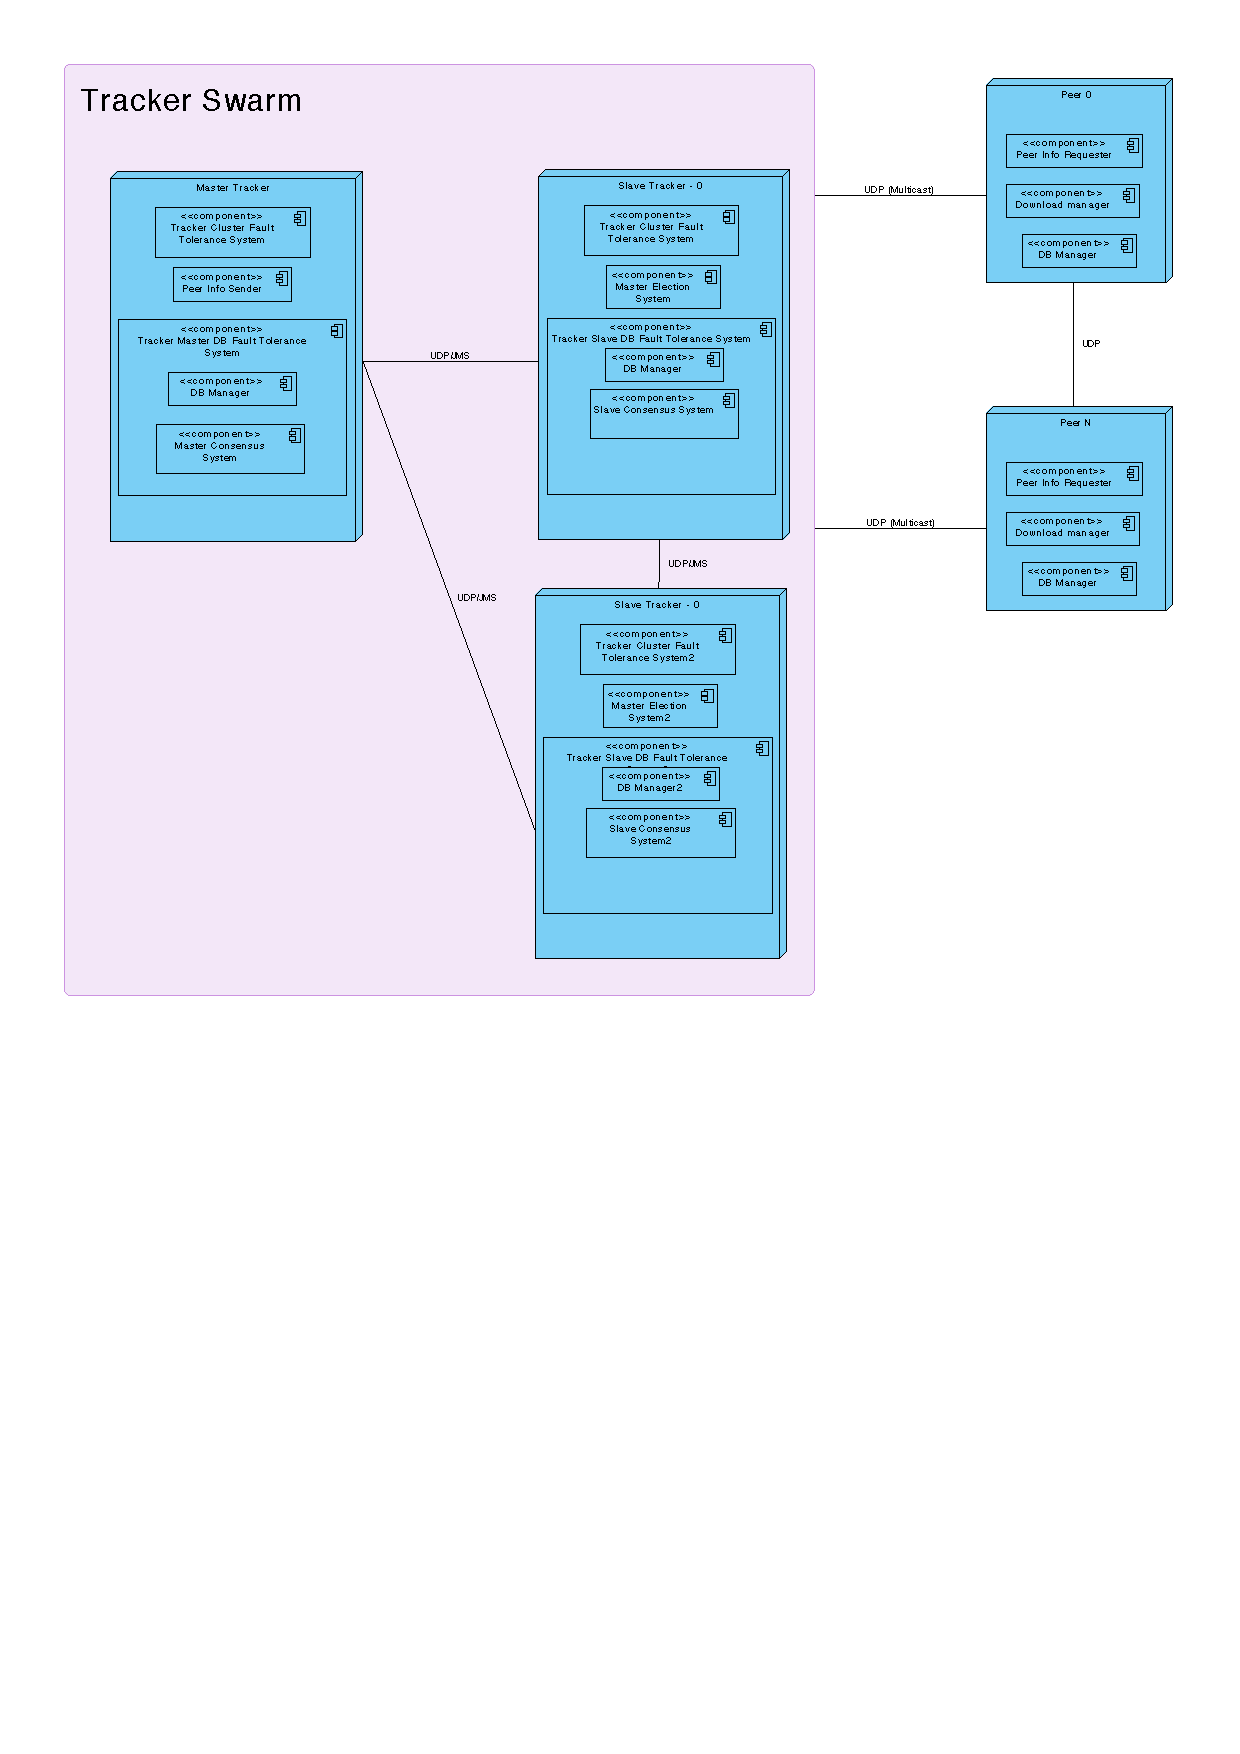
\includegraphics[width=\textwidth]{architectural-design.pdf}
  \caption{\label{fig:arch}Architectural design of the Tracker.}
\end{figure}

\section{Functionality}

The tracker's functionality is summarised in table~\ref{tab:fun-entities}.

\begin{table}
  \centering
  \begin{tabularx}{\linewidth}{l l X}
    Identifier & Entity & Description \\ \hline\hline \\
    Peer Info Sender & Master tracker (MT) & Sends information about the peers and
    the content they have available. \\
    Master DB Fault Tolerance System (M-DFTS) & MT & Composed of the
    \emph{DB Manager} and \emph{Master Consensus System}, ensures that the
    DB is replicated among all the swarm members.\\
    Master Consensus System & MT & This component manages the DB
    replication.\\
    Master Election System & Tracker slaves (TS) & Chooses a new master among the
    slaves when the previous one has fallen.\\
    Slave DB Fault Tolerance System (S-DFTS) & TS & Composed of a
    \emph{DB Manager} and a \emph{Slave Consensus System}, listens to the
    M-DFTS' orders to ensure the DB replication in the slave.\\
    Slave Consensus System & TS &  Ensures the DB replication of
    the slave.\\
    Peer Info Requester & Peers (P) & Requests information about the peers and the
    available contents.\\
    Download Manager & P & This component handles the downloads in the
    clients.\\
    Cluster Fault Tolerance System & MT and TS &
    In charge of sending keep-alive messages among all the members of the
    swarm.\\
    DB Manager & MT, TS and P & Interface with the
    DB system.\\
  \end{tabularx}
  \caption{\label{tab:fun-entities}Summary of the functionality
    implemented in each entity.}
\end{table}

The following list describes more thoroughly the functions previously shown in
table~\ref{tab:fun-entities} that each component is responsible for:

\begin{itemize}
\item Master tracker
  \begin{itemize}
  \item \emph{Cluster Fault Tolerance System}: this component is implemented
    in all the tracker's instances, and it is in charge of knowing the state
    of all the instances. This component sends and receives Keepalive (KA)
    messages from all the instances of the cluster.
    When the master dies sends a
    notification to the \emph{Master Election System} to start the new master
    election process.
  \item \emph{Peer Info Sender}: answers to a client's information request with
    information about the available peers with a specific content.
  \item \emph{Master DB Fault Tolerance System}
    \begin{itemize}
    \item \emph{DB Manager}: handles the Master-Slave database schema described
      at Section~\ref{sec:data-schema}, see figure~\ref{fig:schema-MS}.
    \item \emph{Master Consensus System}: it has two main functions, (i) when a
      DB transaction needs to be propagated among all the instances,
      this component is in charge of coordinating such event by waiting for all
      the instances to be ready, and transmitting the order; (ii) when a
      new slave is created it sends the necessary information to keep its
      DB up to date.
    \end{itemize}
  \end{itemize}
\item Tracker slaves
  \begin{itemize}
  \item \emph{Cluster Fault Tolerance System}: refer to the Master Tracker's
    description of this item.
  \item \emph{Master Election System}: it is notified by the
    \emph{Cluster Fault Tolerance System} about a failure in the Master. This
    component selects a new master among the available slaves. When activated,
    and while the Master election process lasts, the tracker will not listen to
    the clients requests.
  \item \emph{Slave DB Fault Tolerance System}
    \begin{itemize}
    \item \emph{DB Manager}: refer to the Master Tracker's description of this
      item.
    \item \emph{Slave Consensus System}: this component has two functions; on
      the one hand
      (i) when the \emph{Master Consensus System} requests an operation to be
      propagated, checks the slave's status and prepares it to do such
      operation; when the slave is ready, notifies the master, and finally, when
      the master orders to commit, complies. On the other hand, (ii) when the
      slave is a brand-new instance, it requests the latest DB information to
      the master and waits for its instructions to commit.
    \end{itemize}
  \end{itemize}
\item Peers
  \begin{itemize}
  \item \emph{Peer Info Requester}: requests information to the tracker about
    the available peers with some content.
  \item \emph{Download Manager}: manages the download process.
  \item \emph{DB Manager}: handles the Peer database schema described at
    Section~\ref{sec:data-schema}, see figure~\ref{fig:schema-P}.
  \end{itemize}
\end{itemize}


\section{Data schema}\label{sec:data-schema}

Our system contemplates two different database schemas, on the one hand the
tracker's master and slaves will implement the schema shown in
figure~\ref{fig:schema-MS}. This schema has two tables: (i) \texttt{PEER-INFO}
where information regarding the peers' host and ports is stored; and (ii)
\texttt{CONTENTS}, where the tracker will store which peers have available some
specific content. Both tables' fields are self-descriptive.

\begin{figure}[h]
  
  \texttt{PEER-INFO (\underline{id:INTEGER}, host:VARCHAR(255), port:INTEGER)}
  
  \texttt{CONTENTS (\underline{sha1:STRING(40)}, \underline{peer\_id:INTEGER})}
  
  \centering
  \caption{\label{fig:schema-MS}DB schema for the tracker's master and slaves.}
\end{figure}

On the other hand, the peers will need to remember the
progress they have made during a download; thereby, they will store which chucks
they have downloaded so far for a specific file. It must be underlined that our
system will always transfer chunks of the same size, with the exception of the
last chunk, or when the content's size is inferior to our default chunk size.

This characteristic is implemented using the schema shown in
figure~\ref{fig:schema-P}, with the table \texttt{CHUNK}; its
fields are self-descriptive.

\begin{figure}[h]
  
  \texttt{CHUNK (\underline{sha1:STRING(40)}, offset:INTEGER)}
  
  \centering
  \caption{\label{fig:schema-P}DB schema for the tracker's peers.}
\end{figure}

\subsection{DB technology}

We have decided to use SQLite~\cite{sqlite} as our storage technology,
mainly because we have previous experience with it; but more importantly,
because this is a didactic project without the high availability and performance
needs that a professional project's database requires.

Regarding the use of a classic SQL database over the NoSQL paradigm, since
this project implies the synchronisation of the DB over the trackers, we think
that the data should be as normalised as possible and complying to the third
normal form (3NF); thereby, we discard NoSQL databases.

\section{Interaction model design}

\section{Failure model desing}

\section{Graphical interface}


\bibliographystyle{unsrt}
\bibliography{bib}

\end{document}


